% vim: set fileencoding=UTF-8 filetype=tex :
%-----------------------------------------------------------------------------
%
% A 2D state diagramm with bidirectional transitions
%
% Author: Thomas Loruenser (2013): initial version
%
%-----------------------------------------------------------------------------
% Copyright 2013, Thomas Loruenser <thomas.loruenser@ait.ac.at>
%
% This program is free software: you can redistribute it and/or modify
% it under the terms of the GNU General Public License as published by
% the Free Software Foundation, either version 3 of the License, or
% (at your option) any later version.
%
% This program is distributed in the hope that it will be useful,
% but WITHOUT ANY WARRANTY; without even the implied warranty of
% MERCHANTABILITY or FITNESS FOR A PARTICULAR PURPOSE.  See the
% GNU General Public License for more details.
%
% You should have received a copy of the GNU General Public License
% along with this program.  If not, see <http://www.gnu.org/licenses/>.
%-----------------------------------------------------------------------------
\documentclass{standalone}

\usepackage{tikz}
\usetikzlibrary{calc,arrows,positioning}

\begin{document}

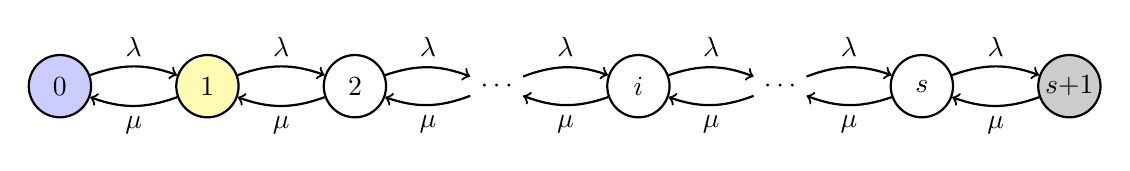
\begin{tikzpicture}[
    node distance=3em,
    thick,
    terminal/.style={
      draw,circle,inner sep=1pt,minimum size=2.25em
    },
    doubletrans/.style={->,bend left=20}
  ]

  \node (s0) [terminal,fill=blue!20!white] at (0,0) 		{$0$};
  \node (s1) [terminal,fill=yellow!30!white,right=of s0] 	{$1$};
  \node (s2) [terminal,right=of s1] 						{$2$};
  \node (s3) [right=of s2]								{$\cdots$};
  \node (s4) [terminal,right=of s3] 						{$i$};
  \node (s5) [right=of s4]								{$\cdots$};
  \node (s6) [terminal,right=of s5] 						{$s$};
  \node (s7) [terminal,fill=gray!40!white,right=of s6] 	{$s$+$1$};

  % draw edges
  \foreach \x in {0,...,6} {
    \pgfmathparse{int(\x+1)}
    \edef\X{\pgfmathresult}
    \draw [doubletrans] (s\x) to node[above] {$\lambda$} (s\X);
    \draw [doubletrans] (s\X) to node[below] {$\mu$}     (s\x);
  }
\end{tikzpicture}

\end{document}
